%!TEX program = <xelatex>
\documentclass[xetex]{beamer}
% \documentclass[draft, xetex]{beamer}
		% Iclude packages and commands used text-wide.	
%%%%%%%%%%%%%%%%%%%%%%%%%%%%%%%%%%%%%%%%%%%%%%%%%%%%%%%%%%%%%%%%%%%%%%%%%%%%%%%%%%%%%%%%%%%%%%%%%%%%%%%%%%%
\usepackage{mystyle}
%%%%%%%%%%%%%%%%%%%%%%%%%%%%%%%%%%%%%%%%%%%%%%%%%%%%%%%%%%%%%%%%%%%%%%%%%%%%%%%%%%%%%%%%%%%%%%%%%%%%%%%%%%%	

	\mode<presentation>{
		%\usetheme{Berlin}
		\usetheme{CambridgeUS}
		\setbeamercovered{transparent}
	}

		% Title
	\title[Mass Spectrometry]{Modelling Mass Spectrometry Data}
	\subtitle{Without any subtitles!}

	%\beamerdefaultoverlayspecification{<+->}
	\date{17 October 2013} 
	\author[Matteo]{Mateusz Łącki}
	\institute[UW]{Uniwersytet Warszawski}
	\titlegraphic{
\includegraphics[scale=.14, keepaspectratio]{./picts/eagle3.png}}
	
	%\usefonttheme[onlylarge]{structuresmallcapsserif}
	%\usefonttheme[onlysmall]{structurebold}

		% The document
%%%%%%%%%%%%%%%%%%%%%%%%%%%%%%%%%%%%%%%%%%%%%%%%%%%%%%%%%%%%%%%%%%%%%%%%%%%%%%%%%%%%%%%%%%%%%%%%%%%%%%%%%%%	

\begin{document}
	\fontspec[Numbers={OldStyle}]{Linux Libertine O}

	%%%%%%%%%%%%%%%%%%%%%%%%%%%%%%%%%%%%%%%%%%%%%%%%%%%%%xetex%%%%%%%%%%%%%


	\begin{frame}\frametitle{Sticks: chemist-friedliness}
		\begin{itemize}
			\item 	Zaniedbujemy różnice w masach dodatkowych neutronów
			\item 	BRAIN $\rightarrow$ generuje $p_R$
			\item 	Problem z budową zmiennej objaśnianej i zmiennych objaśniających
			\begin{itemize}
				\item 	Zmienność w wynikach pomiarów na poziome $0.1$ Th  	
			\end{itemize}
		\end{itemize}
	\end{frame}

	\begin{frame}[plain]
	    \begin{center}
	        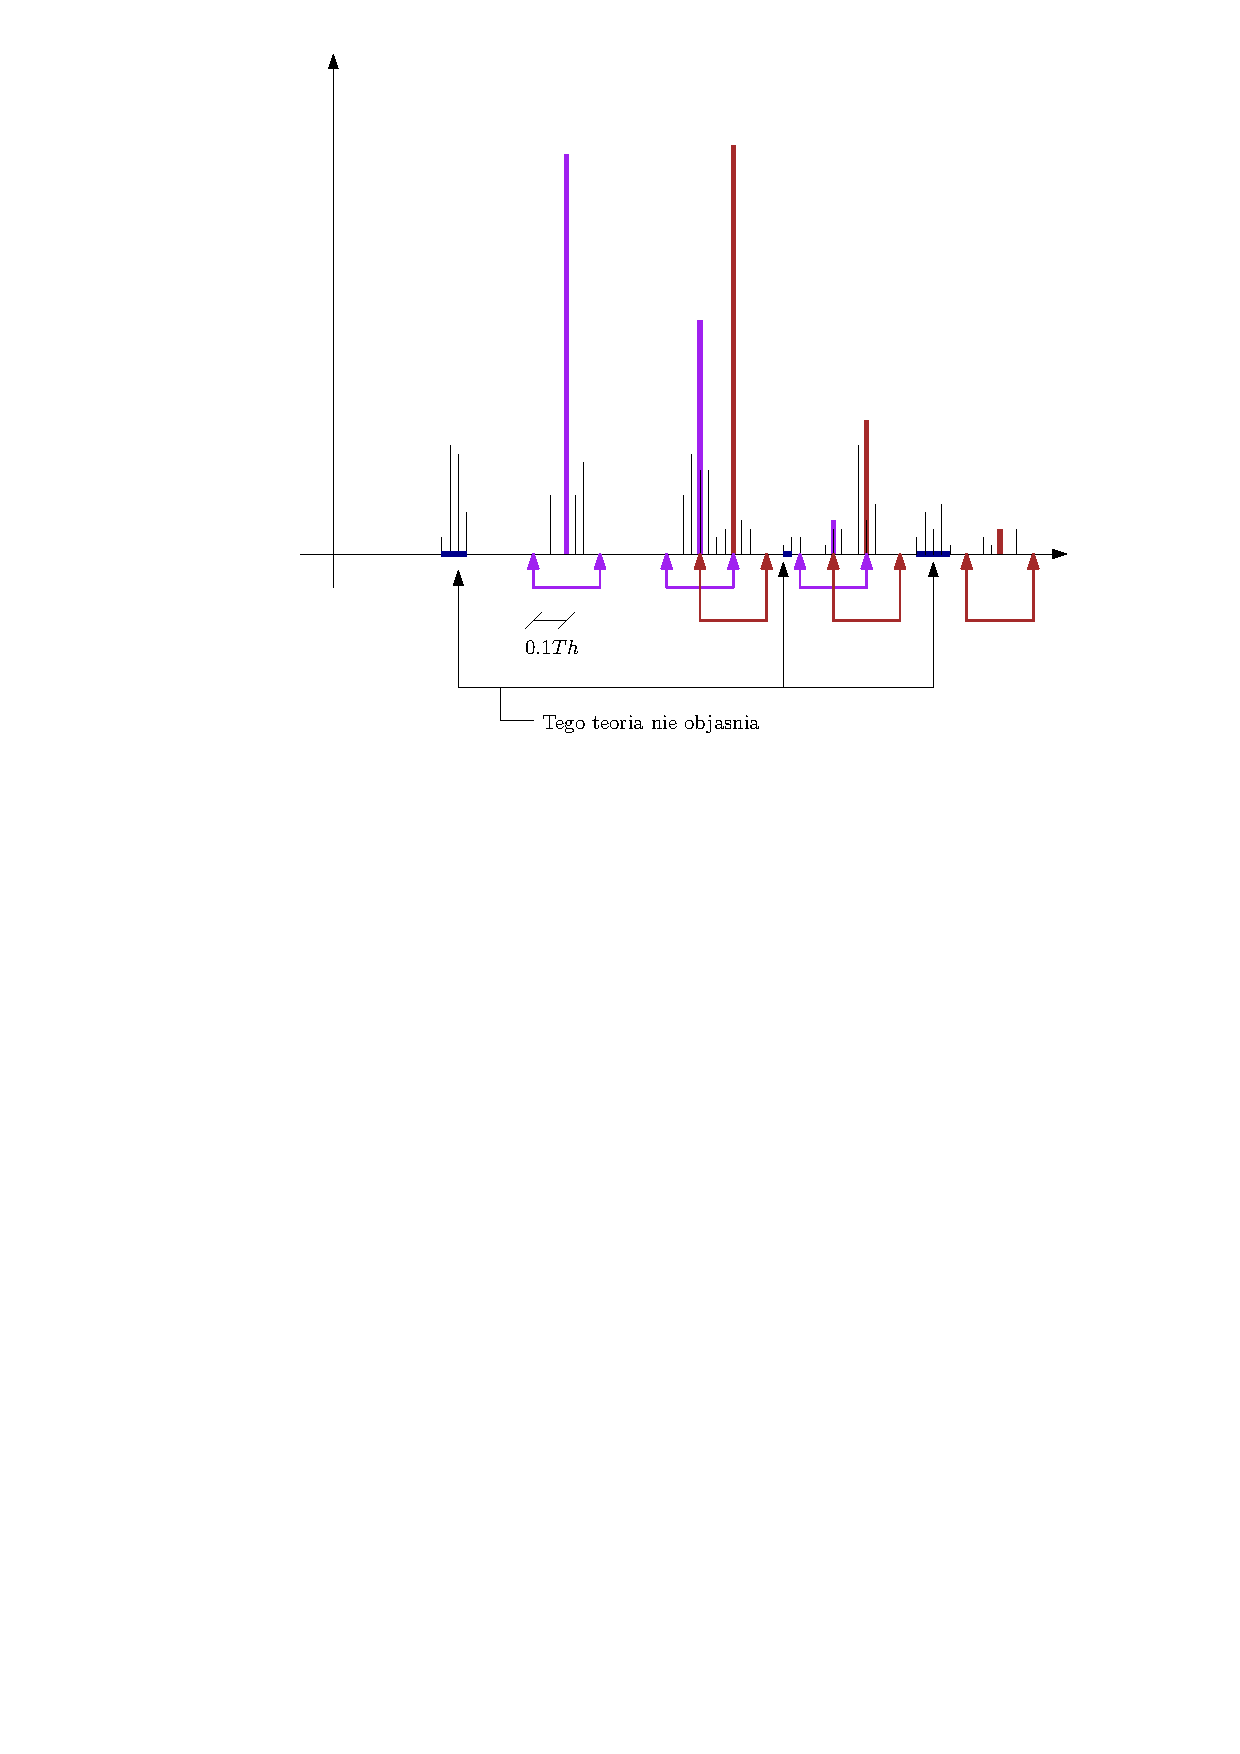
\includegraphics[height=.9\textheight,keepaspectratio]{./picts/sticks}
	    \end{center}
	\end{frame}

	\begin{frame}[plain]
	    \begin{center}
	        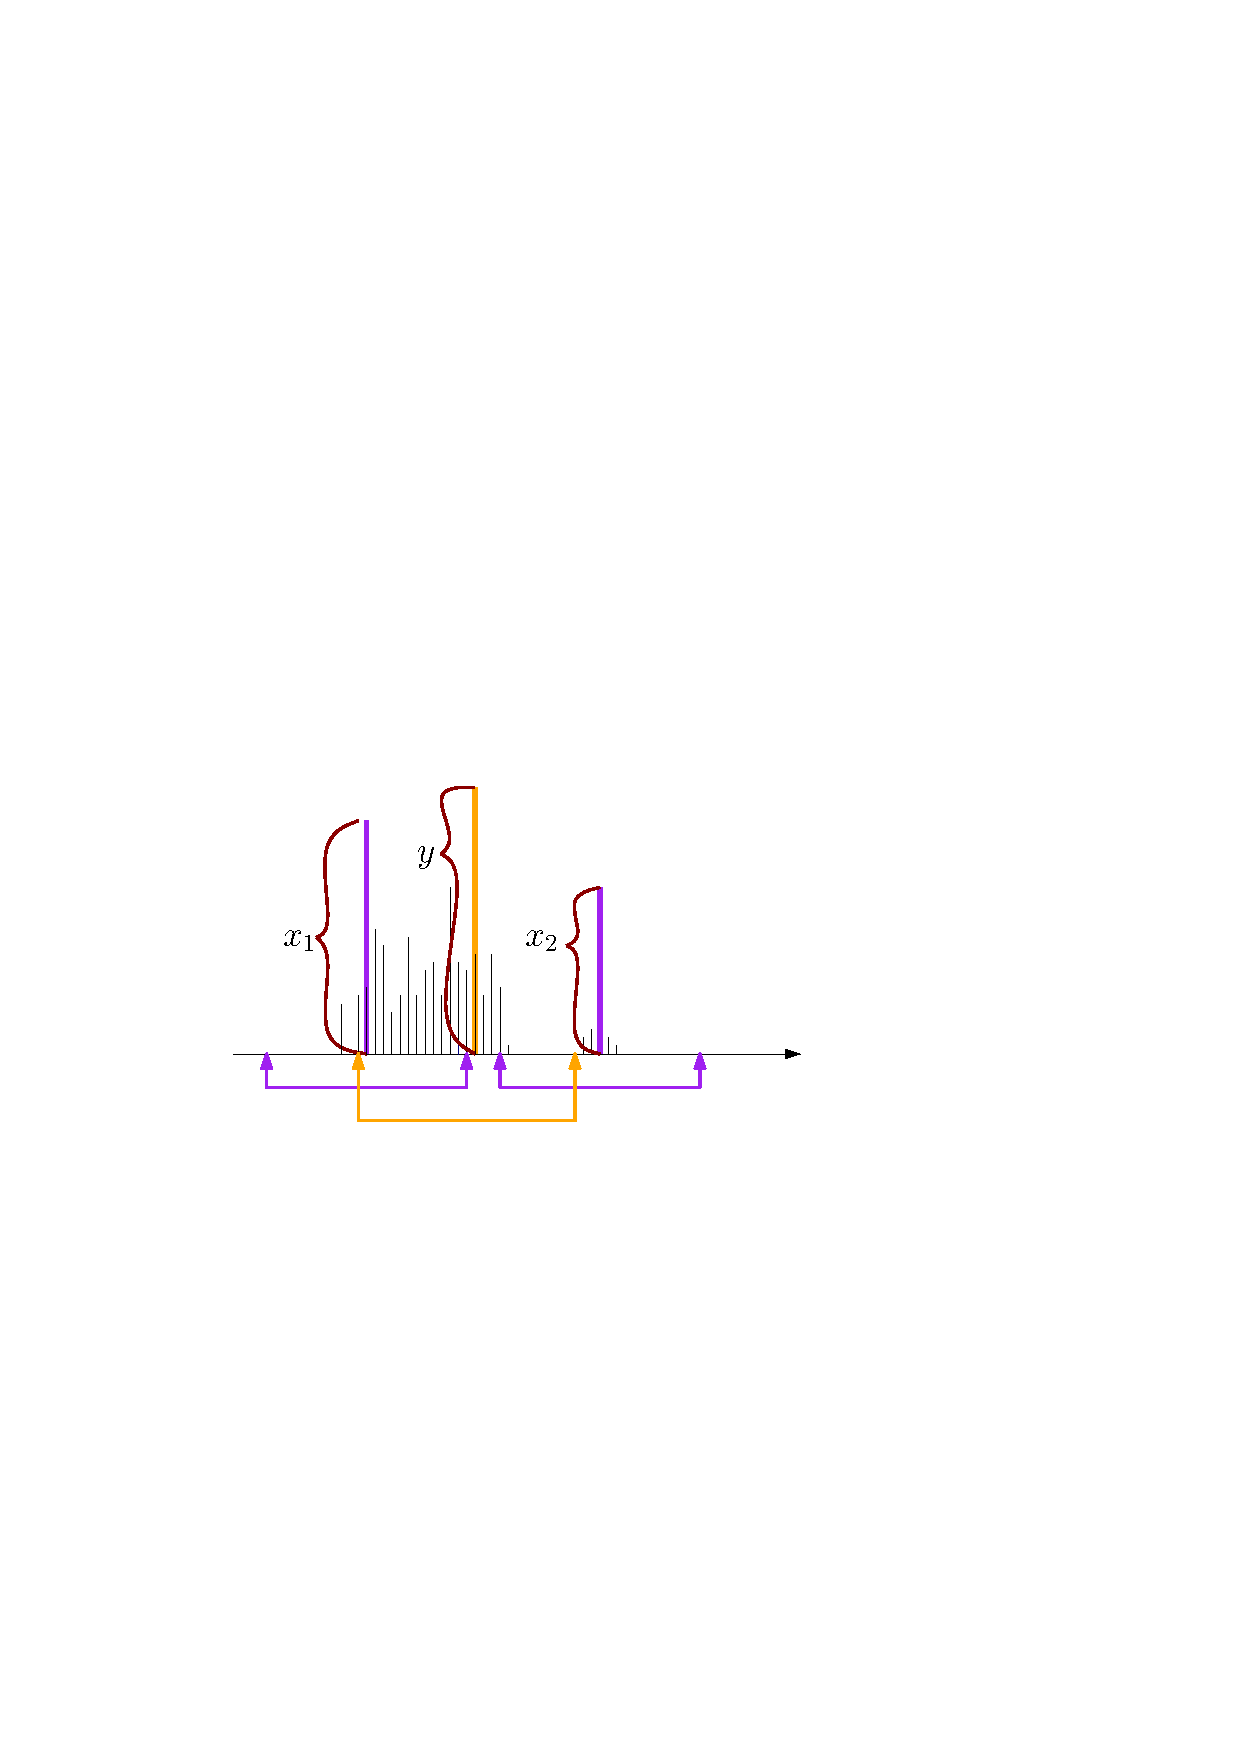
\includegraphics[height=.5\textheight,keepaspectratio]{./picts/sticks2}
	    \end{center}

		\begin{align*}
			z_1 &= \alpha x_1 + \epsilon_1 \\
	    	z_2 &= \alpha x_1 + \beta y + \epsilon_2 \\
	    	z_3 &= \beta x_2 + \epsilon_3 
		\end{align*}

	\end{frame}

	\begin{frame}\frametitle{Problem z patykami}
	    

	    \begin{center}
	        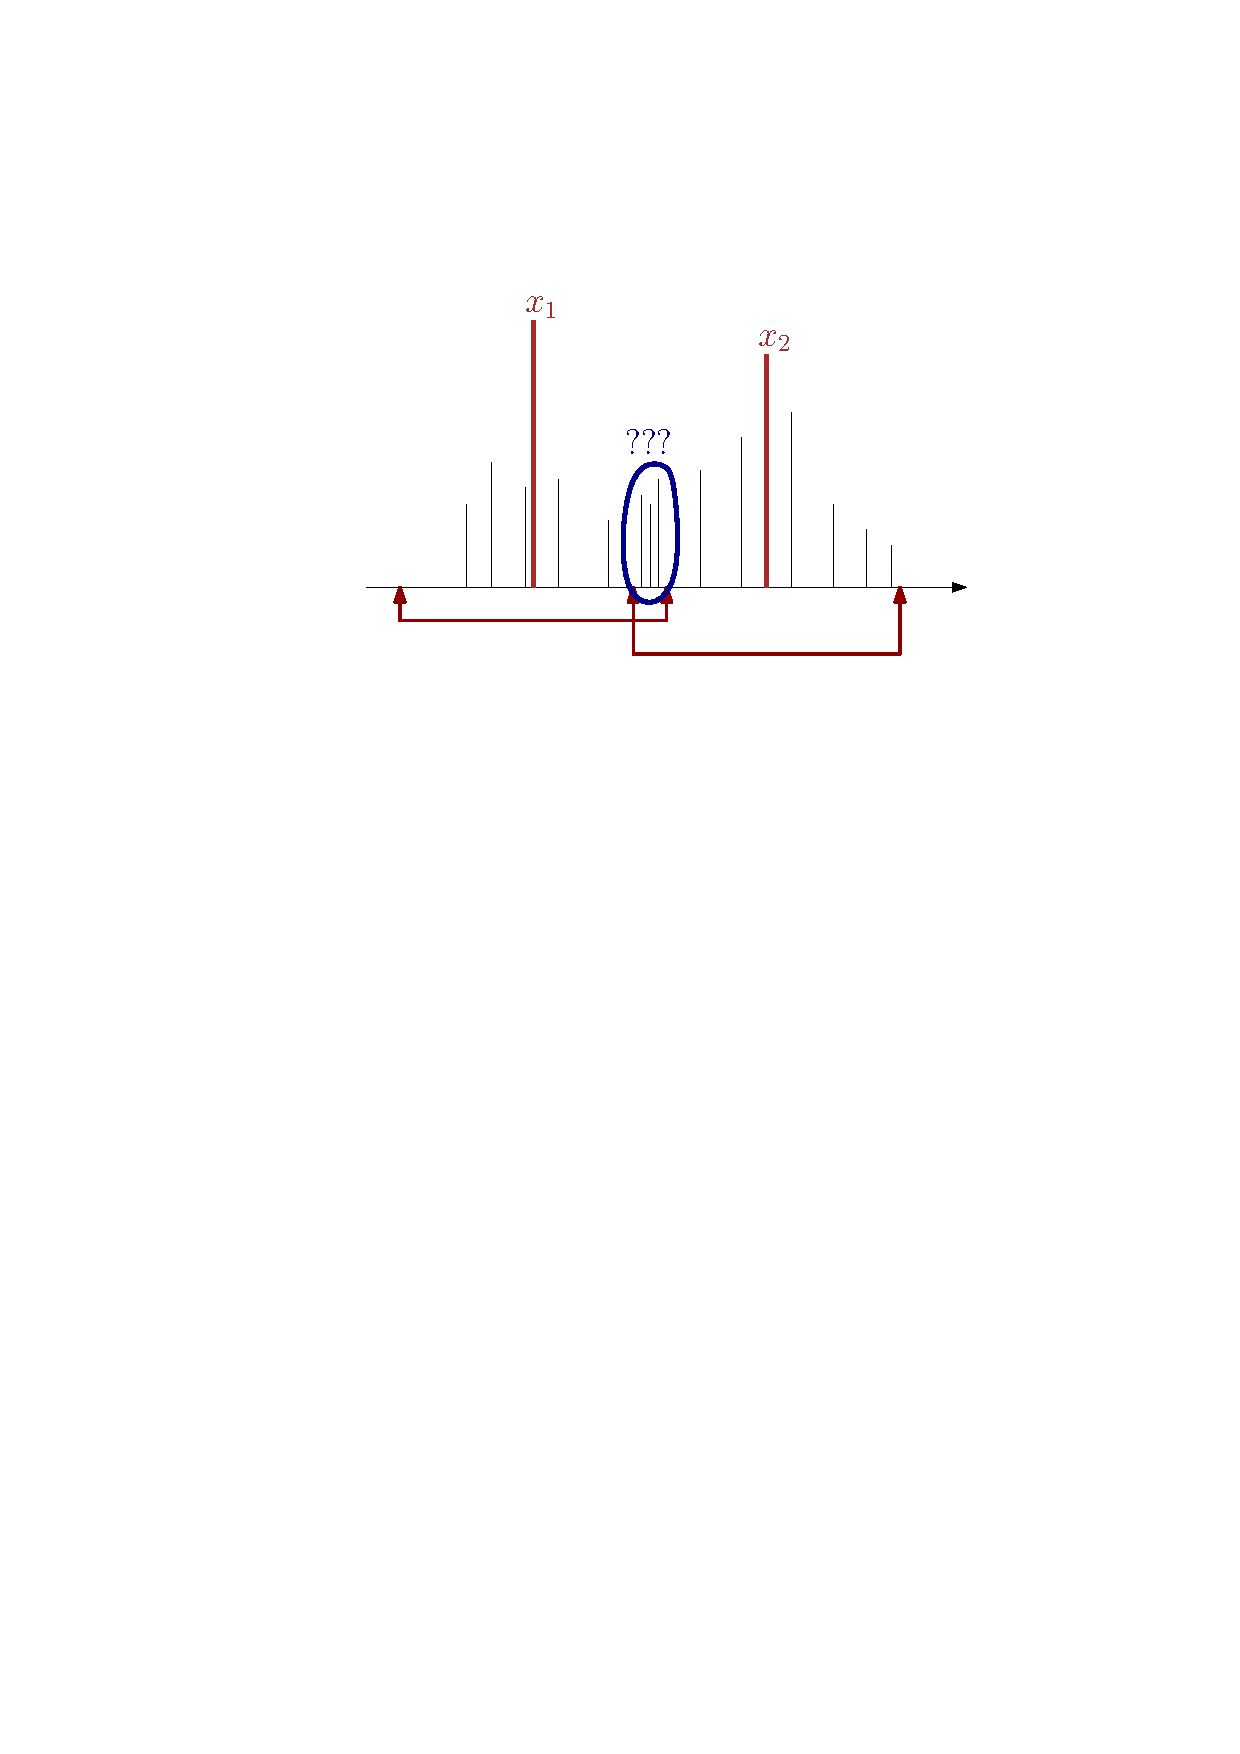
\includegraphics[height=.5\textheight,keepaspectratio]{./picts/sticks3}
	    \end{center}

		\begin{itemize}
			\item Jak klasyfikować spektrum empiryczne w tym przypadku?
		\end{itemize}

	\end{frame}


	\begin{frame}\frametitle{GaussianSticks}
	    

	    \begin{center}
	        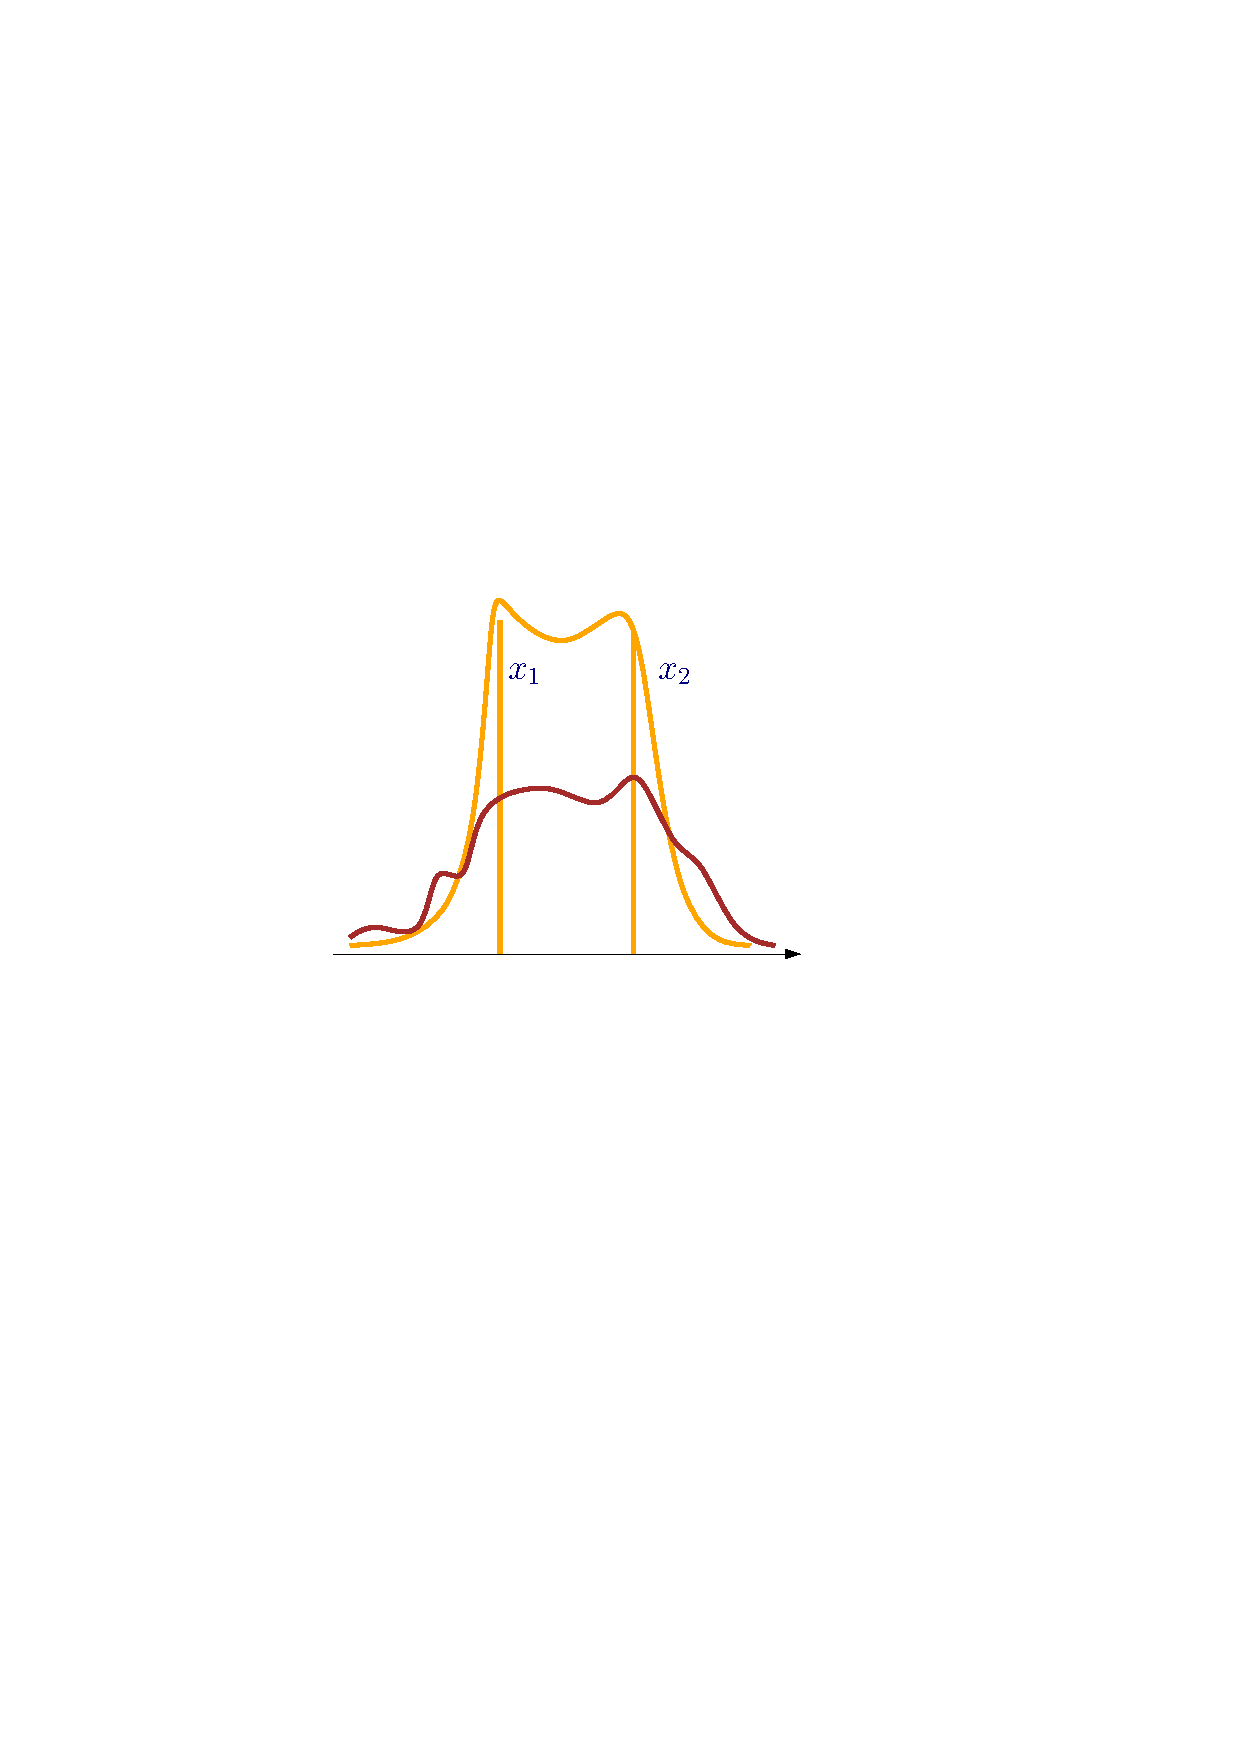
\includegraphics[height=.5\textheight,keepaspectratio]{./picts/sticks4}
	    \end{center}

		\begin{itemize}
			\item Rozmywamy wyniki uzyskane z BRAINa
			$$ f_R (x) = \sum_{\frac{m}{z} \in \text{Nośnik}_R} p_R \Big( \frac{m}{z} \Big) \times g \Biggl( \frac{x-\frac{m}{z}}{\sigma_R} \Biggl) $$
		\end{itemize}

	\end{frame}
\end{document}